\section{Processi primari}

\subsection{Fornitura}
	\subsubsection{Scopo}
	Lo scopo del processo di fornitura è di determinare le procedure e le risorse 
	necessarie allo svolgimento del progetto. Una volta comprese le richieste del 
	proponente e aver stilato uno \textit{Studio di Fattibilità}, il processo può 
	essere avviato con fine di soddisfare ognuna di queste richieste. Inoltre si 
	deve stipulare e concordare con il proponente un contratto per la consegna del 
	prodotto. Si passa dunque a determinare le procedure, le risorse necessarie, e 
	si sviluppa un \textit{Piano di Progetto} che getterà le basi da perseguire fino 
	alla consegna del materiale prodotto.
	Il processo di fornitura è composto dalle seguenti attività che verranno 
	analizzate nell'apposita sezione:
		\begin{itemize}
			\item avvio;
			\item approntamento di risposta alle richieste;
			\item contrattazione;
			\item pianificazione;
			\item esecuzione e controllo;
			\item revisione e valutazione;
			\item consegna e completamento.
		\end{itemize}
	
	\subsubsection{Aspettative} \mbox{}\\ 
	\noindent Il gruppo intende mantenere un costante dialogo con il proponente, per avere un 
	riscontro efficace sul lavoro svolto e instaurare un rapporto di collaborazione 
	per quanto riguarda:
		\begin{itemize}
			\item gli aspetti chiave da determinare per far fronte ai bisogni del proponente;
			\item i requisiti e i vincoli sui processi da stilare;
			\item le tempistiche di lavoro da stimare;
			\item una verifica continua sul lavoro svolto;
			\item eventuali dubbi emersi da chiarire;
			\item accordarsi sulla qualifica del prodotto.
		\end{itemize}
	
	\subsubsection{Descrizione} \mbox{}\\ 
		\noindent Questa sezione tratta le norme che i membri del gruppo \textit{8Lab Solutions} 
		devono rispettare in tutte le fasi di progettazione, sviluppo e consegna del 
		prodotto \textit{Soldino}, al fine di diventare fornitori nei confronti del 
		proponente \textit{Red Babel} e dei committenti Prof. Tullio Vardanega e Prof. 
		Riccardo Cardin.

	\subsubsection{Attività}
		\paragraph{Avvio} \mbox{}\\
		Il fornitore effettua un'analisi dei requisiti in accordo con le politiche 
		organizzative e di altri regolamenti. \\ \\
			\textbf{Studio di Fattibilità} \mbox{}\\ 

			\noindent \'E compito del responsabile di progetto organizzare riunioni tra i membri del 
			gruppo al fine di permettere lo scambio di opinioni sui capitolati proposti.
			Lo \textit{Studio di Fattibilità}, redatto dagli analisti, indica per ogni 
			capitolato\glo:
				\begin{itemize}
					\item \textbf{informazioni generali}: vengono elencate le informazioni di 
						base, come il nome del progetto, il proponente e il committente;
					\item \textbf{descrizione e finalità del progetto}: viene fatta una 
						presentazione del capitolato\glosp in generale, una descrizione delle 
						caratteristiche principali richieste per il prodotto e viene definito 
						l'obiettivo che si vuole raggiungere;
					\item \textbf{tecnologie interessate}: viene fatto un elenco delle tecnologie 
						richieste per lo svolgimento, che rientrano nel dominio tecnologico;
					\item \textbf{aspetti positivi, criticità e fattori di rischio}: vengono 
						esposte le considerazione fatte dal gruppo sugli aspetti positivi e sui fattori 
						di rischio del capitolato\glo;
					\item \textbf{conclusioni}: vengono esposte le ragioni per la quale il gruppo 
						ha deciso di accettare o scartare il capitolato\glo.
				\end{itemize}
		\paragraph{Approntamento di risposte e richieste} \mbox{}\\
		Il fornitore definisce e prepara una proposta in risposta alle richieste del 
		proponente.
		\paragraph{Contrattazione} \mbox{}\\
		Il fornitore negozia e stipula un contratto con il committente per fornire il 
		prodotto o servizio software.
		\paragraph{Pianificazione} \mbox{}\\
		Il fornitore deve sviluppare il piano di gestione del progetto in base ai 
		requisiti e alle opzioni selezionate. \\ \\
			\textbf{Piano di Progetto} \mbox{}\\ 
			
			\noindent Il responsabile, con l'aiuto degli amministratori, redige un 
			\textit{Piano di 
				Progetto} da seguire durante il corso del progetto. Questo documento 
				contiene:
			\begin{itemize}
				\item \textbf{analisi dei rischi}: vengono analizzati nel dettaglio i 
				rischi 
				che potranno presentarsi e vengono esposte le misure e le modalità 
				attraverso le 
				quali i rischi vengono contenuti o mitigati. Viene anche fornita la 
				probabilità 
				con la quale questi possono presentarsi e il livello di gravità per 
				ciascuno;
				\item \textbf{modello di sviluppo\glo}: viene descritto il modello di 
				sviluppo\glosp che è stato scelto, indispensabile per la pianificazione;
				\item \textbf{pianificazione}: vengono pianificate le attività da eseguire 
				nelle diverse fasi del progetto e vengono stabilite le loro scadenze 
				temporali;
				\item \textbf{preventivo e consuntivo}: viene data una stima di lavoro 
				necessaria per ciascuna fase proponendo così un preventivo per il costo 
				totale 
				del progetto. Viene anche tracciato, un consuntivo di periodo relativo 
				all'andamento rispetto a ciò che è stato preventivato.
			\end{itemize} \mbox{}\\
			
			\noindent\textbf{Piano di Qualifica} \mbox{}\\
			
			\noindent I verificatori dovranno redigere un documento, detto \textit{Piano di 
				Qualifica} contenente le strategie da adottare per garantire la qualità del 
			materiale prodotto dal gruppo e dei processi attuati. Il piano è così 
			suddiviso:
			\begin{itemize}
				\item \textbf{qualità di processo}: vengono identificati dei processi dagli 
				standard, stabiliti degli obiettivi, escogitate delle strategie per 
				attuarli e 			
				individuate le metriche per misurarli e controllarli;
				\item \textbf{qualità di prodotto}: vengono identificati gli attributi più 
				rilevanti per il prodotto, definiti degli obiettivi per raggiungerli e 
				delle 
				metriche per misurarli;
				\item \textbf{specifiche dei test}: definiscono una serie di test 
				attraverso 
				i quali il prodotto passa per garantire che soddisfi i requisiti;
				\item \textbf{standard di qualità}: vengono esposti gli standard di qualità 
				scelti;
				\item \textbf{valutazioni per il miglioramento:} vengono riportati i 
				problemi 
				e le relative soluzioni nel ricoprire un determinato ruolo e nell'uso degli 
				strumenti scelti;
				\item \textbf{resoconto delle attività di verifica:} per ogni attività si 
				riportano i risultati delle metriche calcolate in forma di resoconto.
			\end{itemize}

		\paragraph{Esecuzione e controllo} \mbox{}\\
		Il fornitore deve attuare ed eseguire i piani sviluppati nella fase di 
		pianificazione e sviluppare il prodotto software monitorando il progresso e la 
		qualità.
		\paragraph{Revisione e valutazione} \mbox{}\\
		Il fornitore deve eseguire la verifica e validazione al fine di dimostrare che 
		il prodotto software soddisfa i requisiti.
		\paragraph{Consegna e completamento} \mbox{}\\
		Il fornitore consegna il prodotto software come specificato dal contratto.	

		

		
%	\subsubsection{Strumenti}
%	Di seguito sono elencati gli strumenti utilizzati durante il processo di 
%	fornitura.
%	
%		\paragraph{Microsoft Excel} \mbox{}\\ 
%		
%		\noindent Software della suite Microsoft Office per realizzare fogli elettronici. Usato 
%		per fare calcoli, produrre diagrammi, istogrammi e areogrammi, creare tabelle e 
%		grafici.
%				
%		\paragraph{Microsoft Project} \mbox{}\\ 
%		
%		\noindent Per assistere i responsabili di progetto nella pianificazione, 
%		nell'assegnazione delle risorse, nella verifica del rispetto dei tempi, nella 
%		gestione dei budget e nell'analisi dei carichi di lavoro attraverso la creazioni 
%		di diagrammi di Gantt\glo, è stato utilizzato Microsoft Project. \\
%				\centerline{\url{https://products.office.com/it-it/project/}}
%				%PLACEHOLDER
%			\begin{figure}[H]
%				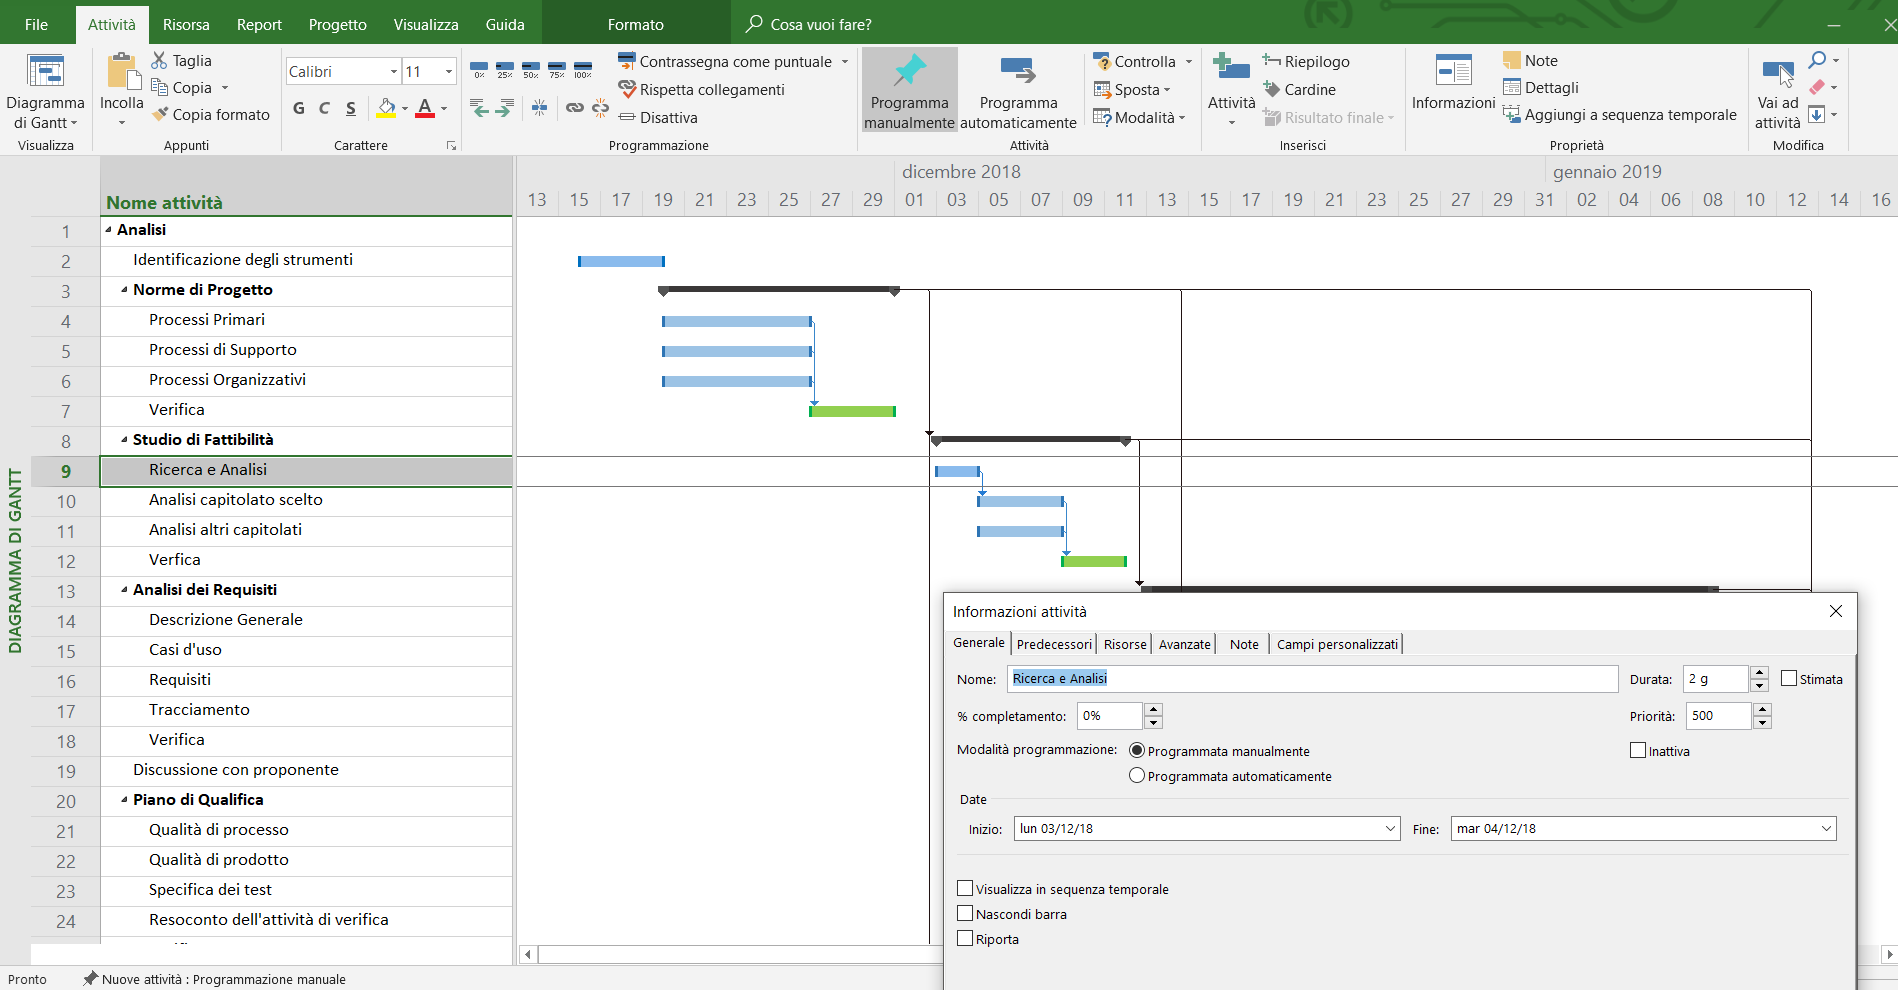
\includegraphics[width=0.99\linewidth]{res/images/projectS.png}
%				\caption{Microsoft Project: Gantt}
%			\end{figure}
			 

		
%\subsubsection{Collaudo e consegna del prodotto}
%Al fine di consegnare il prodotto terminato il gruppo deve effettuare un 
%collaudo in presenza del proponente e dei committenti. Precedentemente a questo 
%test il gruppo deve assicurare correttezza, completezza e affidabilità per ogni 
%parte del materiale consegnato, permettendo così che tutti i requisiti 
%obbligatori siano soddisfatti e l'esecuzione dei test abbiano un esito positivo. 
%In seguito al collaudo finale il responsabile di progetto consegna il prodotto 
%su un supporto fisico.
		
     
\subsection{Sviluppo}

	\subsubsection{Scopo}
	Il processo contiene le attività e i compiti da svolgere, al fine di realizzare 
	il prodotto finale richiesto dal proponente.
	
	\subsubsection{Aspettative}
	Le aspettative sono le seguenti:
		\begin{itemize}
			\item fissare gli obiettivi di sviluppo;
			\item fissare i vincoli tecnologici;
			\item fissare i vincoli di design;
			\item realizzare un prodotto finale che superi i test, che soddisfi i 
				requisiti e le richieste del proponente.
		\end{itemize}
		
	\subsubsection{Descrizione}
	Il processo di sviluppo si articola in:
		\begin{itemize}
			\item analisi dei requisiti;
			\item progettazione;
			\item codifica.
		\end{itemize}
		
	\subsubsection{Attività}
		\paragraph{Analisi dei requisiti}
		\mbox{}\\ \mbox{}\\
			\subparagraph{Scopo}  \mbox{}\\ \mbox{}\\
			Lo scopo dei requisiti è di:
				\begin{itemize}
					\item definire la finalità del lavoro;
					\item considerare lo scopo del progetto e le richieste degli stakeholder;
					\item fissare le funzionalità e i requisiti concordati col cliente;
					\item formulare la definizione di casi d'uso e requisiti;
					\item valutare il corpo dei requisiti e negoziare cambiamenti se necessario;
					\item fornire  una  base  per  raffinamenti  successivi  al  fine  di garantire  un miglioramento continuo del prodotto e del processo di sviluppo;
					\item fornire ai verificatori riferimenti per l'attività di controllo dei test;
					\item calcolare la mole di lavoro per tracciare dei riferimenti per un stima dei costi.
				\end{itemize}
			\subparagraph{Aspettative} \mbox{}\\ \mbox{}\\
			\noindent Obiettivo dell'attività è la creazione della documentazione formale contenente tutti i requisiti richiesti dal proponente. \\ \\		
			\subparagraph{Descrizione} \mbox{}\\ \mbox{}\\
			Durante l'analisi le informazioni ottenute dalle varie fonti sono trasformate in forma di casi d'uso e requisiti. Questa forma fornisce una descrizione dettagliata del sistema e definisce il funzionamento e le caratteristiche di ogni sua parte.\newline
			Gli analisti individuano i requisiti del progetto attraverso lo studio del capitolato, gli incontri con il proponente e i casi d'uso. Tali requisiti sono 	presenti nel documento formale \textit{Analisi dei Requisiti}, in cui viene riportata 	anche la lista dei casi d'uso. \newline
			\noindent I requisiti si raccolgono secondo modalità predefinite:
			\begin{itemize}
				\item lettura del capitolato\glo, analisi e approfondimento dello stesso;
				\item confronto con il proponente;
				\item confronto tra membri del team di progetto;
				\item analisi di uno o più casi d'uso.  \\
			\end{itemize}
			
			\subparagraph{Classificazione dei casi d'uso} \mbox{}\\ \mbox{}\\
			\noindent Ogni caso d'uso viene classificato secondo la seguente notazione: \newline \newline
			\centerline{\textbf{UC[codice\_padre].[codice\_figlio]}} \\
			Dove:
				\begin{itemize}
					\item \textbf{codice\_padre}: numero che identifica univocamente i casi 
						d'uso;
					\item \textbf{codice\_figlio}: numero progressivo che identifica i 
						sottocasi. Può a sua volta includere altri livelli. \\
				\end{itemize}
						%\pagebreak
						%esempio di caso d'uso?(immagine)
			Inoltre per ogni caso d'uso bisogna indicare:
				\begin{itemize}
					\item codice identificativo;
					\item titolo;
					\item diagramma UML\glo;
					\item attori primari;
					\item attori secondari;
					\item descrizione;
					\item scenario principale;
					\item scenario alternativo (se presente);
					\item inclusioni(se presenti);
					\item estensioni(se presenti);
					\item specializzazioni(se presenti);
					\item precondizione;
					\item postcondizione. \\
				\end{itemize}
				
			\subparagraph{Classificazione dei requisiti} \mbox{}\\ \label{sec:UC}
			
			\noindent Ogni requisito viene classificato secondo la seguente notazione: \newline \newline
			\centerline{\textbf{R[Importanza][Tipologia][Codice]}} \\ 
			Dove:
				\begin{itemize}
					\item \textbf{Importanza}: ogni requisito può assumere uno dei seguenti 
						valori:
						\begin{itemize}
							\item \textit{1}: requisito obbligatorio, ovvero irrinunciabile per gli 
								stakeholder;
							\item \textit{2}: requisito desiderabile, ovvero non strettamente 
								necessari ma a valore aggiunto riconoscibile;
							\item \textit{3}: requisito opzionale, ovvero relativamente utile oppure 
								contrattabile più avanti nel progetto.	
						\end{itemize}
					\item \textbf{Tipologia}: ogni requisito può assumere uno dei seguenti 
						valori:
						\begin{itemize}
							\item \textit{F}: funzionale;
							\item \textit{Q}: prestazionale;
							\item \textit{P}: qualitativo;
							\item \textit{V}: vincolo.
						\end{itemize}
					\item \textbf{Codice}: è un identificatore univoco del requisito in forma 
						gerarchica padre/figlio.
				\end{itemize}
				
			\noindent
			Inoltre per ogni requisito bisogna indicare:	
				\begin{itemize}		
					\item \textbf{classificazione}: viene riportata l'importanza del requisito. 
						Sebbene questa sia un'informazione ridondante ne facilita la lettura;
					\item \textbf{descrizione}: descrizione breve ma completa del requisito, 
						meno ambigua possibile;
					\item \textbf{fonti}: ogni requisito può derivare da una o più tra le 
					seguenti opzioni:
					\begin{itemize}
						\item \textit{capitolato\glo}: si tratta di un requisito individuato dalla 
							lettura del capitolato\glo;
						\item \textit{interno}: si tratta di un requisito che gli analisti hanno 
							ritenuto opportuno aggiungere;
						\item \textit{caso d'uso}: il requisito è estrapolato da uno o più casi 
							d'uso. In questo caso deve essere riportato il codice univoco del caso d'uso;
						\item \textit{verbale}: si tratta di un requisito individuato in seguito ad 
							una richiesta di chiarimento con il proponente. Tali informazioni sono riportate 
							nei verbali in cui ogni requisito individuato è segnato da un codice presente 
							nella tabella dei tracciamenti. \\
					\end{itemize}
				\end{itemize}
			
			\subparagraph{Diagrammi UML} \mbox{}\\ \label{sec:UML}
			
			\noindent I diagrammi UML\glosp devono essere realizzati usando la versione del 
			linguaggio v2.0 e per garantirne la leggibilità è necessario:
				\begin{itemize}
					\item distribuire in modo omogeneo gli elementi e possibilmente allinearli 
						sia in senso verticale che in senso orizzontale;
					\item mantenere i margini di spazio tra gli elementi di un gruppo uguali a 
						quelli di gruppi analoghi qualora si hanno le stesse tipologie di elementi;
					\item impostare i collegamenti in uscita da un elemento ad angolo retto. 
				\end{itemize}

			
			\subparagraph{Produzione dei diagrammi UML} \mbox{}\\ \mbox{}\\
			Per la creazione dei casi d'uso utilizziamo il linguaggio UML 2.0.
			Lo strumento adibito alla produzione dei diagrammi è \textbf{Draw.io}.
			Vi si accede tramite Google Drive con le credenziali dell'account google del gruppo.
			In Google Drive, i diagrammi si trovano in \texttt{Analisi dei requisiti > UML Draw.io}.
			Un diagramma UML deve essere creato rispettando il seguente ordine:
			\begin{itemize}
				\item nel menù \texttt{New}, scegliere \texttt{More} e quindi fare
				click \texttt{draw.io Diagrams};
				\item realizzare il diagramma con le convenzioni descritte nel paragrafo precedente; 
				\item nel menù \texttt{File}, scegliere \texttt{Export as..} e selezionare \texttt{PNG};
				\item inserire un nome esplicativo (per es: UC14) e cliccare sull'icona di
				Google Drive;
				\item alla richiesta di selezionare in quale cartella salvare il diagramma 
				in formato PNG selezionare \texttt{No, pic folder..} e assicurarsi di salvare 
				nella cartella apposita denominata \texttt{png} (il percorso è 
				\texttt{Analisi dei requisiti > UML Draw.io > png}).
			\end{itemize}
			Nella cartella \texttt{UML Draw.io} sono presente sia i file .io sia la cartella \texttt{png}
			con gli stessi file in formato .png.
			Questa scelta permette di portare rapidamente delle modifiche ai diagrammi precedentemente disegnati.
			Inoltre, qualora venga effettuata una modifica, l'autore di tale modifica ha il compito di 
			sostituire il file .png aggiornato con quello precedente. 
			
			\subparagraph{Qualità dei requisiti} \mbox{}\\ \mbox{}\\
			In seguito all'analisi dei requisiti in cui si valutano le necessità del proponente,
			vengono schematizzati i requisiti che descrivono il sistema. 
			La specifica dei requisiti deve avere le seguenti qualità:
			\begin{itemize}
			\item evitare le ambiguità fornendo ad ogni requisito una sola interpretazione formale;
			\item garantire la correttezza, ovvero ogni requisito è realmente richiesto e o necessario;
 			\item essere completo, quindi specificare ogni possibili input per ogni funzione richiesta;
 			\item verificare che il sistema realizzi ogni requisito, per questo è necessario che i requisiti non siano
 			ambigui;
			\item evitare che ci sia contraddizione tra i requisiti;
 			\item permettere di modificare facilmente la struttura e lo stile dei requisiti preservando consistenza e completezza;
 			\item mantenere la tracciabilità di ogni requisito per poter monitorare il suo futuro sviluppo.
			\end{itemize}
					
		\paragraph{Progettazione} \mbox{}\\ \mbox{}\\
		\subparagraph{Scopo} \mbox{}\\
			
			\noindent L'attività di progettazione definisce, in funzione dei requisiti specificati 
			nel documento \textit{Analisi dei Requisiti}, le caratteristiche del prodotto 
			software richiesto. Il compito di questa fase è definire una soluzione del 
			problema che sia soddisfacente per tutti gli stakeholder. La progettazione segue 
			il procedimento inverso rispetto all'\textit{Analisi dei Requisiti} che divide 
			il problema in parti per capirne completamente il dominio applicativo. La 
			progettazione, infatti, rimette insieme le parti specificando le funzionalità 
			dei sottosistemi in modo da ricondurre ad un'unica possibile soluzione. \newline 
			
			
			\subparagraph{Aspettative} \mbox{}\\ \mbox{}\\
			\noindent Il processo ha come risultato la realizzazione dell'architettura del sistema così 
			da fornire le istruzioni necessarie ai programmatori per sviluppare il prodotto finito.
			\newline
			
			\subparagraph{Descrizione}  \mbox{}\\ \mbox{}\\
			\noindent Le parti principali sono due:
				\begin{itemize}
					\item \textbf{technology baseline}: contiene le specifiche della 
						progettazione ad alto livello del prodotto e delle sue componenti, l'elenco dei 
						diagrammi UML\glosp che saranno utilizzati per la realizzazione 
						dell'architettura e i test di verifica;
					\item \textbf{product baseline}: dettaglia ulteriormente l'attività di 
						progettazione, integrando ciò che è riportato nella technology baseline. Inoltre 
						definisce i test necessari alla verifica. \newline
				\end{itemize}
			
			
		\subparagraph{Technology baseline} \mbox{}\\ \mbox{}\\
				
			\noindent Redatta dal progettista, dovrà includere:
				\begin{itemize}
					\item \textbf{diagrammi UML\glo}:
					\begin{itemize}
						\item diagrammi dei casi d'uso;
						\item diagrammi delle classi;
						\item diagrammi dei package;
						\item diagrammi di attività;
						\item diagrammi di sequenza.
					\end{itemize}
					\item \textbf{tecnologie utilizzate}: devono essere descritte le tecnologie 
						adottate specificandone l'utilizzo nel progetto, i vantaggi e gli svantaggi;
					\item \textbf{design pattern\glo}: devono essere descritti i design 
						pattern\glosp utilizzati per realizzare l'architettura. Ogni design 
						pattern\glosp deve essere accompagnato da una descrizione ed un diagramma, che 
						ne esponga il significato e la struttura;
					\item \textbf{tracciamento delle componenti}: ogni requisito deve riferirsi 
						al componente che lo soddisfa;
					\item \textbf{test di integrazione}: l'unione delle parti, intese come 
						classi di verifica, permette di verificare che ogni componente del sistema 
						funzioni nella maniera voluta. \newline
				\end{itemize}
						
		\subparagraph{Product baseline} \mbox{}\\ \mbox{}\\
	
			\noindent A carico del progettista c'è anche la product baseline che si sofferma su diversi aspetti tra i quali:
			\begin{itemize}
				\item \textbf{definizione delle classi}: ogni classe deve essere descritta 
					in modo da spiegarne in maniera esaustiva lo scopo e le funzionalità, evitando 
					ridondanze, a tal fine è imperativo l'utilizzo del seguente 
					schema:
					\begin{itemize}
						\item nome;
						\item visibilità;
						\item attributi;
						\item metodi;
						\item breve descrizione che include scopo e 
						funzionalità.
					\end{itemize}
				\item \textbf{test di unità}: devono essere definiti al fine di verificare 
					che le parti funzionino individualmente nel modo stabilito.
			\end{itemize}
			
		\subparagraph{Qualità dell'architettura} \mbox{}\\ \mbox{}\\
		In seguito alla specifica dei requisiti che consolida le funzionalità 
		richieste, viene realizzata l'architettura del sistema. Tale architettura deve 
 		perseguire le seguenti caratteristiche:
 			\begin{itemize}
 				\item sufficienza: l'architettura soddisfa tutti i requisiti; 
 				\item  modularità: l'architettura è suddivisa in parti ben 
					distinte;
				\item robustezza: l'architettura può sopportare diversi ingressi dall'utente e 
					dall'ambiente;
				\item affidabilità: l'architettura garantisce una buona usabilità del prodotto 
					quando viene implementata;
				\item manutenibilità: l'architettura può subire modifiche a costi contenuti.
 			\end{itemize}
 		
 		In particolare, riguardo alla modularità, il progettista deve scomporre il sistema in
 		moduli, fornendo una descrizione precisa della struttura modulare e delle relazioni 
 		che esistono tra essi. Questo porta ai seguenti vantaggi:
 			\begin{itemize}
 				\item maggiore leggibilità e riusabilità del codice;
 				\item semplificazione dell'individuazione e della correzione degli errori;
 				\item possibilità di realizzazione di prototipi.
 			\end{itemize}
 		   
		Per perseguire le qualità sopra elencate, è richiesta l'implementazione di design pattern
		ove necessario. 
		\newline
		
		Al fine di implementare le qualità dell'architettura appena descritte, 
		ai progettisti viene richiesto di seguire le seguenti regole:
			\begin{itemize}
				\item evitare package vuoti, classi e parametri non utilizzati e parametri senza tipo;
				\item evitare la presenza di dipendenze circolari;
				\item evitare modifiche ai servizi offerti dalle librerie esterne utilizzate;
				\item utilizzare ove possibile interfacce e classi astratte;
				\item utilizzare nomi significativi per le classi e i metodi in esse contenuti, 
					in modo da facilitare la comprensione immediata di ogni componente;
				\item assegnare ad ogni metodo e attributo la visibilità strettamente necessaria.
			\end{itemize}
	
		\paragraph{Codifica}
			\mbox{}\\ \mbox{}\\
			\noindent\textbf{Scopo} \mbox{}\\
	
			\noindent{Questa attività ha come obiettivo normare l'effettiva realizzazione 
			del 
			prodotto software richiesto. In questa fase si concretizza la soluzione 
			attraverso la programmazione. I programmatori dovranno attenersi a queste norme 
			durante la fase di programmazione ed implementazione.} \newline
						
			\noindent\textbf{Aspettative} \mbox{}\\
			
			\noindent{Obiettivo dell'attività è la creazione di un prodotto software conforme alle 
			richieste prefissate con il proponente.
			L'uso di norme e convenzioni in questa fase, è fondamentale per permettere la 
			generazione di codice leggibile ed uniforme,  agevolare le fasi di manutenzione, 
			verifica e validazione e migliorare la qualità di prodotto.} \newline 
			
			\noindent\textbf{Descrizione} \mbox{}\\
			
			\noindent{La scrittura del codice dovrà rispettare quanto stabilito nella 
			documentazione di prodotto. Dovrà perseguire gli obiettivi di qualità definiti 
			all'interno del documento \textit{Piano di Qualifica v4.0.0} per 
			poter garantire 
			una buona qualità del codice.} \newline 
			
			\noindent\textbf{Stile di codifica} \mbox{}\\
			
			\noindent{Al fine di garantire uniformità, leggibilità e manutenibilità del codice del progetto,
			ciascun membro del gruppo è tenuto a rispettare le seguenti norme:}
				\begin{itemize}
					\item \textbf{indentazione}: i blocchi innestati devono essere correttamente 
						indentati, usando per ciascun livello di indentazione quattro (4) spazi (fanno 
						eccezione i commenti). Al fine di assicurare il rispetto di questa regola si 
						consiglia di configurare adeguatamente il proprio editor o IDE;
					\item \textbf{parentesizzazione}: è richiesto di inserire 
					le parentesi di delimitazione dei costrutti in linea e non 
					al di sotto di essi, separando le parentesi con uno spazio;
					\item \textbf{scrittura dei metodi}: è preferibile, ove possibile, 
						mantenere i metodi brevi (poche righe di codice);
					\item \textbf{univocità dei nomi}: classi, metodi, variabili devono avere un 
						nome univoco	ed esplicativo al fine di evitare ambiguità e incomprensione;
					\item \textbf{classi}: i nomi delle classi devono iniziare sempre con una 
						lettera maiuscola;		
					\item \textbf{costanti}: i nomi delle costanti devono essere scritti usando 
						solo maiuscole;
					\item \textbf{metodi}: i nomi dei metodi devono iniziare con una lettera 
						minuscola. Nel caso siano composti da più parole, quelle successive devono iniziare con una 
						lettera maiuscola (CamelCase\glo{});
					\item \textbf{commenti}: deve essere presente un sintetico commento descrittivo precedente all'implementazione di metodi e classi;
					\item \textbf{intestazione dei file}: ogni file deve presentare le seguenti informazioni:
						\begin{itemize}
							\item percorso e nome del file;
							\item nome e cognome dell'autore;
							\item data di creazione;
							\item data ultima modifica;
							\item breve descrizione del contenuto del file.
						\end{itemize}
					\item \textbf{lingua}: il codice, come anche i commenti, deve essere scritto 
						in lingua inglese.
				\end{itemize}
			Una parte del front-end\glosp è normata dalla \href{https://github.com/airbnb/javascript/blob/master/README.md}{Airbnb JavaScript Style Guide}, il cui uso è implementato attraverso ESLint\glo.\newline
			Il back-end è scritto invece seguendo la \href{https://solidity.readthedocs.io/en/v0.5.7/style-guide.html}{Style Guide} presente nella documentazione ufficiale di Solidity.
			 \newline \newline
			%\subparagraph{Intestazione} \mbox{}\\
			\noindent\textbf{Ricorsione}  \mbox{}\\
			
			\noindent{L'uso della ricorsione va evitato quanto più possibile in  quanto potrebbe
			indurre ad una maggiore occupazione di memoria rispetto a soluzioni iterative.}
			
			
			
	\subsubsection{Metriche}
	Illustriamo a seguire le metriche utilizzate nel processo di sviluppo, divise per attività.
		\paragraph{Metriche di analisi dei requisiti}
		\begin{itemize}
			\item \textbf{percentuale di requisiti obbligatori soddisfatti}:
			La percentuale di requisiti obbligatori soddisfatti (PROS) mostra la percentuale di requisiti soddisfati sui requisiti totali, e viene calcolata con la seguente formula:	
			\begin{center}
				$ PROS = \frac{requisiti\ obbligatori\ soddisfatti}{requisiti\ obbligatori\ totali}$
			\end{center}		
		\end{itemize}		
		\paragraph{Metriche di progettazione}
		\begin{itemize}
			\item \textbf{accoppiamento tra le classi di oggetti}:
			l'accoppiamento tra classi e oggetti (CBO) indica se una classe è accoppiata ad una seconda, cioè se la prima usa metodi o variabili definiti nella seconda. Si calcola con un un valore intero.
		\end{itemize}
		\paragraph{Metriche di codifica}
			\begin{itemize}
				\item \textbf{Numero di variabili di stato per contratto}: considera il numero totale di variabili di stato presenti all'interno di un contratto. Un valore elevato può indicare, oltre a un costo elevato dovuto all'alto numero di attributi, che tale contratto si fa carico di una quantità eccessiva di responsabilità; potrebbe quindi convenire scorporare una parte di esso in un secondo contratto;
				\item \textbf{Livello di annidamento}: il livello di annidamento nei vari metodi tenendo	conto della presenza di strutture di controllo annidate.  Un alto livello di annidamento porta a un codice di difficile manutenzione, aumentandone la complessità; potrebbe quindi convenire scorporare il metodo in più metodi distinti;
				\item \textbf{Profondità della gerarchica}: la profondità della gerarchia va limitata in modo da limitare l'accoppiamento;
				\item \textbf{Numero di parametri per metodo}: un numero troppo elevato di parametri in un metodo potrebbe indicare un grado di complessità troppo elevato del metodo. In Solidity\glo, per motivi di ottimizzazione dei costi il numero di parametri per funzione deve essere al più 10.
			\end{itemize}
			
	\subsubsection{Strumenti}
	Di seguito sono elencati gli strumenti utilizzati dal gruppo durante il 
	progetto per il processo di sviluppo.
			
		\paragraph{ESLint} \mbox{}\\ \mbox{}\\
		Utilità open-source per scrivere codice JavaScript secondo regole di codifica 
		predeterminate. Esegue segnalazioni su patterns presenti nel codice 
		ECMAScript/JavaScript.\\
		\centerline{\url{https://eslint.org/}}
				
		\paragraph{PragmaDB} \mbox{}\\ \mbox{}\\
		Programma usato per il tracciamento dei requisiti, fondamentale dunque 
		per la stesura del documento \textit{Analisi dei Requisiti v3.0.0}. 
		\newline
		\centerline{\url{https://github.com/StefanoMunari/PragmaDB}}
			\begin{figure}[H]
				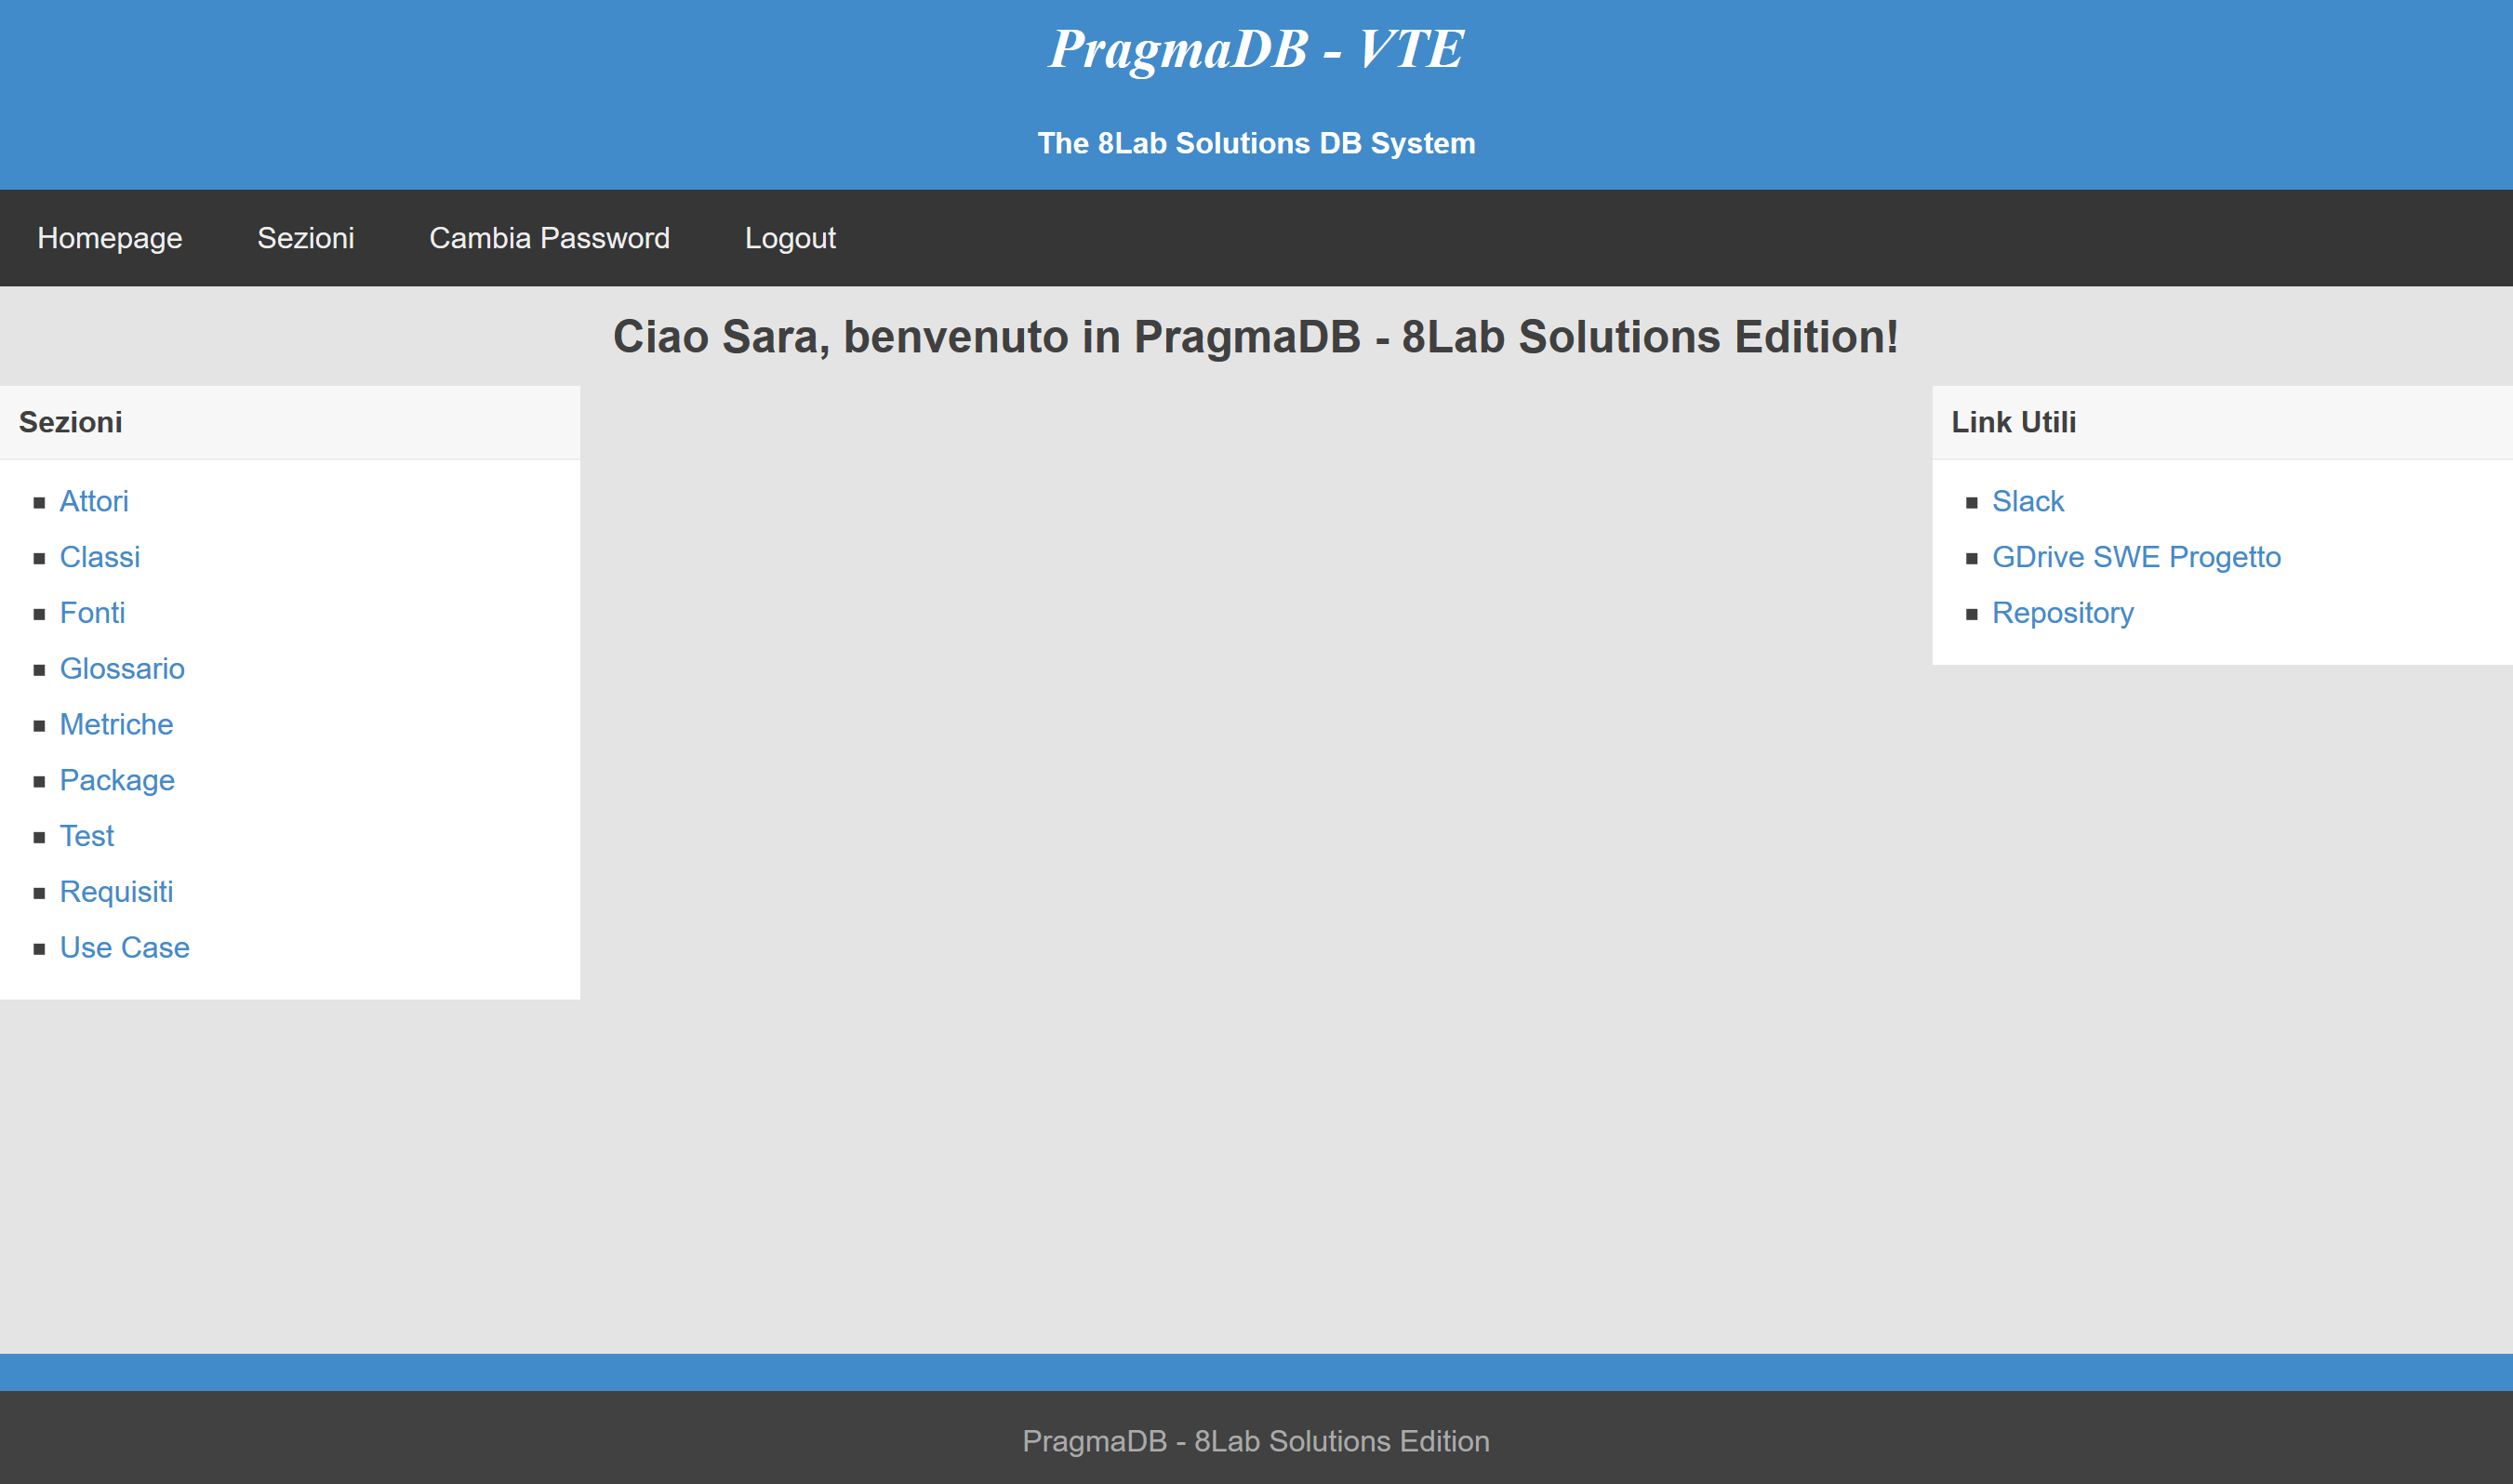
\includegraphics[width=0.99\linewidth]{res/images/HomepagePragmaDB.png}
				\caption{Homepage PragmaDB di un utente autenticato}
			\end{figure}

		\paragraph{Draw.io} \mbox{}\\ \mbox{}\\
		Per la produzione di diagrammi UML\glosp viene utilizzato Draw.io in quanto 
		offre molte agevolazioni per la produzione veloce dei diagrammi e risulta 
		semplice da usare. \newline
		\centerline{\url{https://www.draw.io/}}
			\begin{figure}[H]
				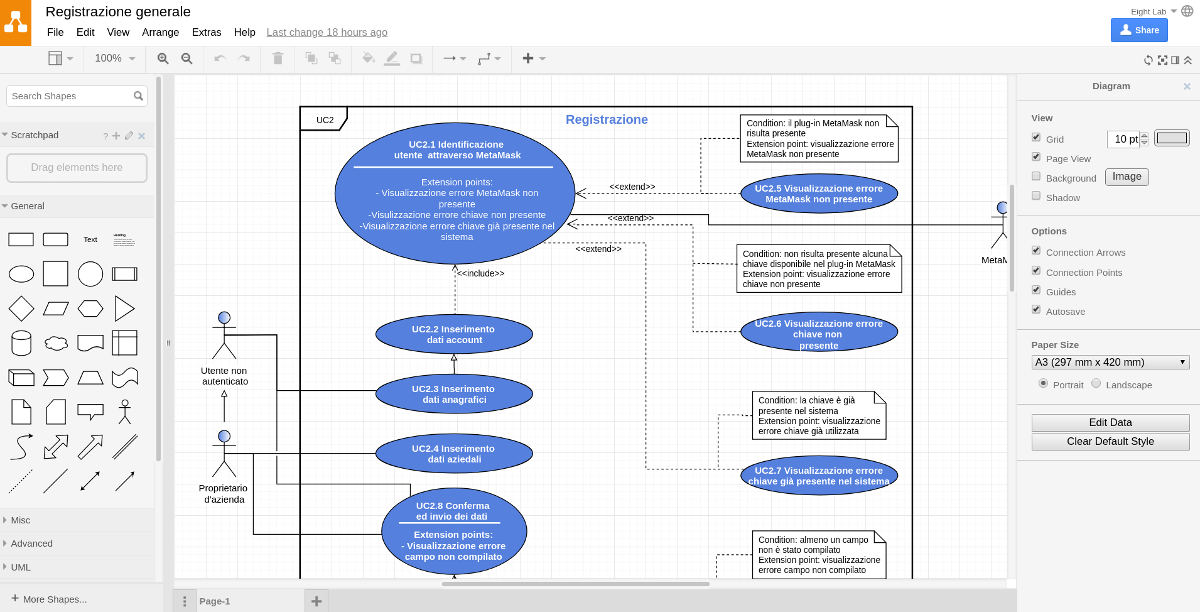
\includegraphics[width=0.99\linewidth]{res/images/drawio.jpg}
				\caption{Software per la creazione di diagrammi online}
			\end{figure} 
				
		\paragraph{Visual Studio Code} \mbox{}\\ \mbox{}\\
		Visual Studio Code viene utilizzato per la codifica in Solidity, Java e JavaScript. Questo 
		IDE offre piena compatibilità con Linux, Windows, macOS, oltre ad essere un 
		potente editor con molte funzionalità integrate. \newline
		\centerline{\url{https://code.visualstudio.com/}}
			\begin{comment}
				\begin{figure}[H]
					\includegraphics[width=0.99\linewidth]{res/images/""}
					\caption{Software per la codifica}
				\end{figure} 
			\end{comment}
			
		\paragraph{Truffle} \mbox{}\\ \mbox{}\\
		Per lo sviluppo, test e gestione di smart contracts\glo, permette la scrittura automatizzata di test in JavaScript e Solidity\glo.\newline
		\centerline{\url{https://truffleframework.com/truffle}}
		
		\paragraph{React} \mbox{}\\ \mbox{}\\ 
		Per la realizzazione dell'interfaccia utente a livello di applicazione web.\newline
		\centerline{\url{https://reactjs.org/}}
		
		\paragraph{Solidity} \mbox{}\\ \mbox{}\\ 
		Per lo sviluppo di smart contracts\glo, tale linguaggio viene impiegato in Visual Studio Code.\newline
		\centerline{\url{https://solidity.readthedocs.io/en/v0.5.3/}}
		
		\paragraph{MetaMask} \mbox{}\\ \mbox{}\\ 
		Utilizzato per effettuare transazioni sicure sulla rete Ethereum\glosp senza ospitare un nodo della rete e per eseguire ÐApps\glo. \newline
		\centerline{\url{https://metamask.io/}}
		
		\paragraph{Ganache} \mbox{}\\ \mbox{}\\
		Impiegato per simulare una blockchain\glosp Ethereum\glosp locale.\\
		\centerline{\url{https://truffleframework.com/ganache}}
		
		\paragraph{Sass} \mbox{}\\ \mbox{}\\
		Utilizzato per generare file CSS ottimizzati.\\
		\centerline{\url{https://sass-lang.com/}}
		
		\paragraph{Web3} \mbox{}\\ \mbox{}\\
		Utilizzato per fare interagire il livello di back end\glosp con quello di front end\glo. \\
		\centerline{\url{https://web3js.readthedocs.io/en/1.0/}}
		
		\paragraph{Redux} \mbox{}\\ \mbox{}\\
		Utilizzato per mantenere lo stato dell'applicazione.\\
		\centerline{\url{https://redux.js.org/}}
		
		\paragraph{Travis} \mbox{}\\ \mbox{}\\
		Impiegato per garantire la continuous integration.\\
		\centerline{\url{https://travis-ci.org/}}
		
		\paragraph{Surge.sh} \mbox{}\\ \mbox{}\\
		Utilizzato per favorire l'accessibilità del sito a livello globale, ovvero occupa la posizione di host dell'applicazione.\\
		\centerline{\url{https://surge.sh/}}
		
		\paragraph{Node.js} \mbox{}\\ \mbox{}\\
		Utilizzato per creare applicazioni di rete scalabili non solo lato client ma anche lato server.\\
		\centerline{\url{https://nodejs.org/it/about/}}
		
		\paragraph{NPM} \mbox{}\\ \mbox{}\\
		Utilizzato per poter installare i pacchetti necessari allo sviluppo dell'applicativo, quali React\glo, Redux\glo, Truffle\glo, Ganache CLI\glosp e Web3\glo. \\
		\centerline{\url{https://www.npmjs.com/}}
		
		\paragraph{IPFS} \mbox{}\\ \mbox{}\\
		InterPlanetary File System, \'e un protocollo progettato per la condivisione di file e documenti attraverso un file system 
		distribuito e con un approccio peer-to-peer. \\
		\centerline{\url{https://ipfs.io/}}
		
		\paragraph{Infura} \mbox{}\\ \mbox{}\\
		Utilizzato per effettuare l'accesso in modo sicuro e affidabile a IPFS\glo. \\
		\centerline{\url{https://infura.io/}}
		
%	\subsection{Procedure}	
%	% PRAGMA
%	\subsubsection{PragmaDB} 
%	Per eseguire le seguenti operazioni è necessario eseguire la login al sito 
%\\
%	
%\centerline{\url{http://ec2-52-47-35-145.eu-west-3.compute.amazonaws.com/PragmaDB/PHP/}}
%	in cui ogni membro del gruppo deve inserire username e password.
%	
%	\paragraph{Aggiungere un attore} \mbox{}\\ \mbox{}\\
%	Dopo aver eseguito l'autenticazione:
%	\begin{itemize}
%		\item selezionare \texttt{Attori} nel pannello posto a sinistra;
%		\item selezionare \texttt{Inserisci Attore} nel panello posto a destra;
%		\item compilare il form per l'inserimento di un nuovo attore, inserendo 
%		il nome e la descrizione relativi ad esso;
%		\item cliccare sul tasto \texttt{Conferma} per aggiungere il nuovo 
%attore 
%		creato oppure \texttt{Cancella} per tornare indietro.	
%	\end{itemize}
%	
%	\paragraph{Modificare un attore} \mbox{}\\ \mbox{}\\
%	Dopo aver eseguito l'autenticazione:
%	\begin{itemize}
%		\item selezionare \texttt{Attori} nel pannello posto a sinistra;
%		\item selezionare \texttt{Modifica} dalla riga della tabella dell'attore
%		che si vuole modificare;
%		\item modificare i campi del form dell'attore selezionato;
%		\item cliccare sul tasto \texttt{Modifica} per salvare le modifiche 
%effettuate
%		oppure \texttt{Cancella} per tornare indietro.	
%	\end{itemize}
%	
%	\paragraph{Eliminare un attore} \mbox{}\\ \mbox{}\\
%	Dopo aver eseguito l'autenticazione:
%	\begin{itemize}
%		\item selezionare \texttt{Attori} nel pannello posto a sinistra;
%		\item selezionare \texttt{Elimina} dalla riga della tabella dell'attore
%		che si vuole eliminare;
%		\item cliccare sul tasto \texttt{Elimina} per confermare la rimozione
%		oppure \texttt{Cancella} per tornare indietro.	
%	\end{itemize}
%	
%	\paragraph{Aggiungere una classe} \mbox{}\\ \mbox{}\\
%	Dopo aver eseguito l'autenticazione:
%	\begin{itemize}
%		\item selezionare \texttt{Classi} nel pannello posto a sinistra;
%		\item selezionare \texttt{Inserisci Classe} nel panello posto a destra;
%		\item compilare il form per l'inserimento di una nuova classe;
%		\item cliccare sul tasto \texttt{Inserisci} per aggiungere la nuova 
%classe 
%		creata oppure \texttt{Cancella} per tornare indietro.	
%	\end{itemize}
%	
%	\paragraph{Modificare una classe} \mbox{}\\ \mbox{}\\
%	Dopo aver eseguito l'autenticazione:
%	\begin{itemize}
%		\item selezionare \texttt{Classi} nel pannello posto a sinistra;
%		\item selezionare \texttt{Modifica} dalla riga della tabella della 
%classe
%		che si vuole modificare;
%		\item modificare i campi del form della classe selezionata;
%		\item cliccare sul tasto \texttt{Modifica} per salvare le modifiche 
%effettuate
%		oppure \texttt{Cancella} per tornare indietro.
%	\end{itemize}
%	
%	\paragraph{Eliminare una classe} \mbox{}\\ \mbox{}\\
%	Dopo aver eseguito l'autenticazione:
%	\begin{itemize}
%		\item selezionare \texttt{Classi} nel pannello posto a sinistra;
%		\item selezionare \texttt{Eliminare} dalla riga della tabella della 
%classe
%		che si vuole eliminare;
%		\item cliccare sul tasto \texttt{Elimina} per confermare la rimozione 
%della classe
%		oppure \texttt{Annulla} per tornare indietro.
%	\end{itemize}
%	
%	\paragraph{Aggiungere un attributo alla classe} \mbox{}\\ \mbox{}\\
%	Dopo aver eseguito l'autenticazione:
%	\begin{itemize}
%		\item selezionare \texttt{Classi} nel pannello posto a sinistra;
%		\item selezionare \texttt{Attributi} dalla riga della tabella della 
%classe
%		a cui si vuole aggiungere un attributo;
%		\item selezionare \texttt{Inserisci Attributo} dal pannello posto a 
%destra;
%		\item compilare il form per l'inserimento di un nuovo attributo;
%		\item cliccare sul tasto \texttt{Inserisci} per aggiungere il nuovo 
%attributo 
%		creato oppure \texttt{Cancella} per tornare indietro.	
%	\end{itemize}
%	
%	\paragraph{Modificare un attributo alla classe} \mbox{}\\ \mbox{}\\
%	Dopo aver eseguito l'autenticazione:
%	\begin{itemize}
%		\item selezionare \texttt{Classi} nel pannello posto a sinistra;
%		\item selezionare \texttt{Attributi} dalla riga della tabella della 
%classe
%		a cui si vuole modificare un attributo;\
%		\item selezionare \texttt{Modifica} dalla riga della tabella 
%dell'attributo
%		che si vuole modificare;
%		\item modificare i campi del form dell'attributo selezionato;
%		\item cliccare sul tasto \texttt{Modifica} per salvare le modifiche 
%effettuate
%		oppure \texttt{Cancella} per tornare indietro.
%	\end{itemize}
%	
%	\paragraph{Eliminare un attributo alla classe} \mbox{}\\ \mbox{}\\
%	Dopo aver eseguito l'autenticazione:
%	\begin{itemize}
%		\item selezionare \texttt{Classi} nel pannello posto a sinistra;
%		\item selezionare \texttt{Attributi} dalla riga della tabella della 
%classe
%		a cui si vuole eliminare un attributo;\
%		\item selezionare \texttt{Eliminare} dalla riga della tabella 
%dell'attributo 
%		che si vuole eliminare;
%		\item cliccare sul tasto \texttt{Elimina} per confermare la rimozione 
%dell'attributo
%		oppure \texttt{Annulla} per tornare indietro.
%	\end{itemize}
%	
%	\paragraph{Aggiungere un metodo alla classe} \mbox{}\\ \mbox{}\\
%	Dopo aver eseguito l'autenticazione:
%	\begin{itemize}
%		\item selezionare \texttt{Classi} nel pannello posto a sinistra;
%		\item selezionare \texttt{Metodi} dalla riga della tabella della classe
%		a cui si vuole aggiungere un metodo;
%		\item selezionare \texttt{Inserisci Metodo} dal pannello posto a destra;
%		\item compilare il form per l'inserimento di un nuovo metodo;
%		\item cliccare sul tasto \texttt{Inserisci} per aggiungere il nuovo 
%metodo 
%		creato oppure \texttt{Cancella} per tornare indietro.	
%	\end{itemize}
%	
%	\paragraph{Modificare un metodo alla classe} \mbox{}\\ \mbox{}\\
%	Dopo aver eseguito l'autenticazione:
%	\begin{itemize}
%		\item selezionare \texttt{Classi} nel pannello posto a sinistra;
%		\item selezionare \texttt{Metodi} dalla riga della tabella della classe
%		a cui si vuole modificare un metodo;
%		\item selezionare \texttt{Inserisci Metodo} dal pannello posto a destra;
%		\item modificare i campi del form del metodo selezionato;
%		\item cliccare sul tasto \texttt{Modifica} per salvare le modifiche 
%effettuate
%		oppure \texttt{Cancella} per tornare indietro.	
%	\end{itemize}
%	
%	\paragraph{Eliminare un metodo alla classe} \mbox{}\\ \mbox{}\\
%	Dopo aver eseguito l'autenticazione:
%	\begin{itemize}
%		\item selezionare \texttt{Classi} nel pannello posto a sinistra;
%		\item selezionare \texttt{Attributi} dalla riga della tabella della 
%classe
%		a cui si vuole eliminare un metodo;\
%		\item selezionare \texttt{Eliminare} dalla riga della tabella del metodo
%		che si vuole eliminare;
%		\item cliccare sul tasto \texttt{Elimina} per confermare la rimozione 
%del metodo
%		oppure \texttt{Annulla} per tornare indietro.
%	\end{itemize}
%	
%	\paragraph{Aggiungere un requisito alla classe} \mbox{}\\ \mbox{}\\
%	Dopo aver eseguito l'autenticazione:
%	\begin{itemize}
%		\item selezionare \texttt{Classi} nel pannello posto a sinistra;
%		\item selezionare \texttt{Requisiti} dalla riga della tabella della 
%classe
%		a cui si vuole aggiungere un requisito;
%		\item selezionare \texttt{Inserisci Requisito} dal pannello posto a 
%destra;
%		\item compilare il form per l'inserimento di un nuovo metodo;
%		\item cliccare sul tasto \texttt{Inserisci} per aggiungere il nuovo 
%requisito 
%		creato oppure \texttt{Cancella} per tornare indietro.	
%	\end{itemize}
%	
%	\paragraph{Modificare un requisito alla classe} \mbox{}\\ \mbox{}\\
%	Dopo aver eseguito l'autenticazione:
%	\begin{itemize}
%		\item selezionare \texttt{Classi} nel pannello posto a sinistra;
%		\item selezionare \texttt{Requisiti} dalla riga della tabella della 
%classe
%		a cui si vuole modificare un requisito;
%		\item selezionare \texttt{Inserisci Requisito} dal pannello posto a 
%destra;
%		\item modificare i campi del form del requisito selezionato;
%		\item cliccare sul tasto \texttt{Modifica} per salvare le modifiche 
%effettuate
%		oppure \texttt{Cancella} per tornare indietro.
%	\end{itemize}
%	
%	\paragraph{Eliminare un requisito alla classe} \mbox{}\\ \mbox{}\\
%	Dopo aver eseguito l'autenticazione:
%	\begin{itemize}
%		\item selezionare \texttt{Classi} nel pannello posto a sinistra;
%		\item selezionare \texttt{Requisiti} dalla riga della tabella della 
%classe
%		a cui si vuole eliminare un requisito;\
%		\item selezionare \texttt{Eliminare} dalla riga della tabella del 
%requisito
%		che si vuole eliminare;
%		\item cliccare sul tasto \texttt{Elimina} per confermare la rimozione 
%del requisito
%		oppure \texttt{Annulla} per tornare indietro.
%	\end{itemize}
%	
%	\paragraph{Aggiungere una fonte} \mbox{}\\ \mbox{}\\
%	Dopo aver eseguito l'autenticazione:
%	\begin{itemize}
%		\item selezionare \texttt{Fonti} nel pannello posto a sinistra;
%		\item selezionare \texttt{Inserisci Fonte} dal pannello posto a destra;
%		\item compilare il form per l'inserimento di una nuova fonte;
%		\item cliccare sul tasto \texttt{Inserisci} per aggiungere la nuova 
%fonte 
%		creata oppure \texttt{Cancella} per tornare indietro.	
%	\end{itemize}
%	
%	\paragraph{Modificare una fonte} \mbox{}\\ \mbox{}\\
%	Dopo aver eseguito l'autenticazione:
%	\begin{itemize}
%		\item selezionare \texttt{Fonti} nel pannello posto a sinistra;
%		\item selezionare \texttt{Modifica} dalla riga della tabella della fonte
%		che si vuole modificare;
%		\item modificare i campi del form della fonte selezionata;
%		\item cliccare sul tasto \texttt{Modifica} per salvare le modifiche 
%effettuate
%		oppure \texttt{Cancella} per tornare indietro.
%	\end{itemize}
%	
%	\paragraph{Eliminare una fonte} \mbox{}\\ \mbox{}\\\\
%	Dopo aver eseguito l'autenticazione:
%	\begin{itemize}
%		\item selezionare \texttt{Fonti} nel pannello posto a sinistra;
%		\item selezionare \texttt{Elimina} dalla riga della tabella della fonte 
%		che si vuole eliminare;\
%		\item cliccare sul tasto \texttt{Elimina} per confermare la rimozione 
%della fonte
%		oppure \texttt{Annulla} per tornare indietro.
%	\end{itemize}
%	
%	\paragraph{Aggiungere un package} \mbox{}\\ \mbox{}\\
%	Dopo aver eseguito l'autenticazione:
%	\begin{itemize}
%		\item selezionare \texttt{Package} nel pannello posto a sinistra;
%		\item selezionare \texttt{Inserisci Package} dal pannello posto a 
%destra;
%		\item compilare il form per l'inserimento di un nuovo package;
%		\item cliccare sul tasto \texttt{Inserisci} per aggiungere il nuovo 
%package
%		creato oppure \texttt{Cancella} per tornare indietro.	
%	\end{itemize}
%	
%	\paragraph{Modificare un package} \mbox{}\\ \mbox{}\\
%	Dopo aver eseguito l'autenticazione:
%	\begin{itemize}
%		\item selezionare \texttt{Package} nel pannello posto a sinistra;
%		\item selezionare \texttt{Modifica} dalla riga della tabella del package
%		che si vuole modificare;
%		\item modificare i campi del form del package selezionato;
%		\item cliccare sul tasto \texttt{Modifica} per salvare le modifiche 
%effettuate
%		oppure \texttt{Cancella} per tornare indietro.
%	\end{itemize}
%	
%	\paragraph{Eliminare un package} \mbox{}\\ \mbox{}\\
%	Dopo aver eseguito l'autenticazione:
%	\begin{itemize}
%		\item selezionare \texttt{Package} nel pannello posto a sinistra;
%		\item selezionare \texttt{Elimina} dalla riga della tabella del package 
%		che si vuole eliminare;\
%		\item cliccare sul tasto \texttt{Elimina} per confermare la rimozione 
%del package
%		oppure \texttt{Annulla} per tornare indietro.
%	\end{itemize}
%	
%	\paragraph{Aggiungere un test} \mbox{}\\ \mbox{}\\
%	Dopo aver eseguito l'autenticazione:
%	\begin{itemize}
%		\item selezionare \texttt{Test} nel pannello posto a sinistra;
%		\item selezionare \texttt{Inserisci Test} dal pannello posto a destra;
%		\item compilare il form per l'inserimento di un nuovo test;
%		\item cliccare sul tasto \texttt{Inserisci} per aggiungere il nuovo test
%		creato oppure \texttt{Cancella} per tornare indietro.	
%	\end{itemize}
%	
%	\paragraph{Modificare un test} \mbox{}\\ \mbox{}\\
%	Dopo aver eseguito l'autenticazione:
%	\begin{itemize}
%		\item selezionare \texttt{Test} nel pannello posto a sinistra;
%		\item selezionare \texttt{Modifica} dalla riga della tabella del test
%		che si vuole modificare;
%		\item modificare i campi del form del test selezionato;
%		\item cliccare sul tasto \texttt{Modifica} per salvare le modifiche 
%effettuate
%		oppure \texttt{Cancella} per tornare indietro.
%	\end{itemize}
%	
%	\paragraph{Eliminare un test} \mbox{}\\ \mbox{}\\
%	Dopo aver eseguito l'autenticazione:
%	\begin{itemize}
%		\item selezionare \texttt{Test} nel pannello posto a sinistra;
%		\item selezionare \texttt{Elimina} dalla riga della tabella del test
%		che si vuole eliminare;\
%		\item cliccare sul tasto \texttt{Elimina} per confermare la rimozione 
%del test
%		oppure \texttt{Annulla} per tornare indietro.
%	\end{itemize}		
%	
%	\paragraph{Aggiungere un requisito} \mbox{}\\ \mbox{}\\
%	Dopo aver eseguito l'autenticazione:
%	\begin{itemize}
%		\item selezionare \texttt{Requisiti} nel pannello posto a sinistra;
%		\item selezionare \texttt{Inserisci Requisiti} dal pannello posto a 
%destra;
%		\item compilare il form per l'inserimento di un nuovo requisito;
%		\item cliccare sul tasto \texttt{Inserisci} per aggiungere il nuovo 
%requisito
%		creato oppure \texttt{Cancella} per tornare indietro.	
%	\end{itemize}
%	
%	\paragraph{Modificare un requisito} \mbox{}\\ \mbox{}\\
%	Dopo aver eseguito l'autenticazione:
%	\begin{itemize}
%		\item selezionare \texttt{Requisiti} nel pannello posto a sinistra;
%		\item selezionare \texttt{Modifica} dalla riga della tabella del 
%requisito
%		che si vuole modificare;
%		\item modificare i campi del form del requisito selezionato;
%		\item cliccare sul tasto \texttt{Modifica} per salvare le modifiche 
%effettuate
%		oppure \texttt{Cancella} per tornare indietro.
%	\end{itemize}
%	
%	\paragraph{Eliminare un requisito} \mbox{}\\ \mbox{}\\
%	Dopo aver eseguito l'autenticazione:
%	\begin{itemize}
%		\item selezionare \texttt{Requisiti} nel pannello posto a sinistra;
%		\item selezionare \texttt{Elimina} dalla riga della tabella del 
%requisito 
%		che si vuole eliminare;\
%		\item cliccare sul tasto \texttt{Elimina} per confermare la rimozione 
%del requisito
%		oppure \texttt{Annulla} per tornare indietro.
%	\end{itemize}
%	
%	\paragraph{Aggiungere un use case} \mbox{}\\ \mbox{}\\
%	Dopo aver eseguito l'autenticazione:
%	\begin{itemize}
%		\item selezionare \texttt{Use Case} nel pannello posto a sinistra;
%		\item selezionare \texttt{Inserisci Use Case} dal pannello posto a 
%destra;
%		\item compilare il form per l'inserimento di un nuovo use case;
%		\item cliccare sul tasto \texttt{Inserisci} per aggiungere il nuovo use 
%case
%		creato oppure \texttt{Cancella} per tornare indietro.	
%	\end{itemize}
%	
%	\paragraph{Modificare un use case} \mbox{}\\ \mbox{}\\
%	Dopo aver eseguito l'autenticazione:
%	\begin{itemize}
%		\item selezionare \texttt{Use Case} nel pannello posto a sinistra;
%		\item selezionare \texttt{Modifica} dalla riga della tabella del use 
%case
%		che si vuole modificare;
%		\item modificare i campi del form del use case selezionato;
%		\item cliccare sul tasto \texttt{Modifica} per salvare le modifiche 
%effettuate
%		oppure \texttt{Cancella} per tornare indietro.
%	\end{itemize}
%	
%	\paragraph{Eliminare un use case} \mbox{}\\ \mbox{}\\
%	Dopo aver eseguito l'autenticazione:
%	\begin{itemize}
%		\item selezionare \texttt{Use Case} nel pannello posto a sinistra;
%		\item selezionare \texttt{Elimina} dalla riga della tabella del use 
%case 
%		che si vuole eliminare;\
%		\item cliccare sul tasto \texttt{Elimina} per confermare la rimozione 
%del use case
%		oppure \texttt{Annulla} per tornare indietro.
%	\end{itemize}

	
